\question{1.7}{Een groep van dertig eerstejaarsstudenten is een aantal vragen voorgelegd. Dit betrof:
    \begin{itemize}
        \item Leeftijd
        \item Woonsituatie (z=zelfstandig, o=bij ouders)
        \item Geslacht (m=man, v=vrouw)
        \item De maandelijke bestedingen aan voedsel en drank
        \item De score voor het tentamen statistiek
    \end{itemize}
    In het boek staan de resultaten in een tabel beschreven.
}

\begin{enumerate}[label=(\alph*)]
    \item Geef aan op welk type schaal de vijf variabelen worden gemeten
    \answer{Naam: nominaal, leeftijd: ratio, woonsituatie: nominaal, geslacht: nominaal, besteding: ratio, score: ratio}

    \item Maak een frequentieverdeling van de leeftijden
    \answer{
        \begin{center}
            \begin{tabular}{cc}
                \toprule
                    {\bfseries Leeftijd} & {\bfseries Frequentie} \\
                \midrule
                    $18$ & $2$ \\
                    $19$ & $5$ \\
                    $20$ & $6$ \\
                    $21$ & $6$ \\
                    $22$ & $5$ \\
                    $23$ & $3$ \\
                    $24$ & $1$ \\
                    $25$ & $1$ \\
                    $26$ & $1$ \\
                \midrule    
                    Totaal & $30$ \\
                \bottomrule
            \end{tabular}
        \end{center}
    }
    \item Teken een histogram van de bestedingen. Begin met ondergrens \euro 250.
    \answer{
        \begin{center}
            \resizebox{0.9\textwidth}{!}{
                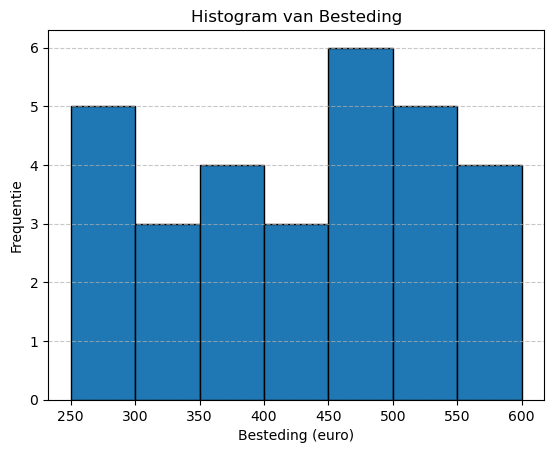
\includegraphics{opg1.7c.png}
            }
        \end{center}
    }
    \item Maak een klassenindeling van de scores voor mannen en vrouwen afzonderlijk. 
    Kies voor de klassen 10 eenheden en verwerk de resultaten in een kruistabel. 
    Bereken ook de procentuele frequenties van de scoreklassen voor de mannen en vrouwen afzonderlijk.
    \answer{
        De absolute frequentieverdeling van de scoreklassen naar geslacht is gelijk aan

        \begin{center}
            \begin{tabular}{ccc|c}
                \toprule
                    {\bfseries Scoreklasse} & {\bfseries Man} & {\bfseries Vrouw} & {\bfseries Totaal} \\
                \midrule
                    $[30, 40)$ & $1$ & $0$ & $1$ \\
                    $[40, 50)$ & $1$ & $5$ & $6$ \\
                    $[50, 60)$ & $3$ & $0$ & $3$ \\
                    $[60, 70)$ & $4$ & $2$ & $6$ \\
                    $[70, 80)$ & $2$ & $4$ & $6$ \\
                    $[80, 90)$ & $4$ & $1$ & $5$ \\
                    $[90, 100)$ & $3$ & $0$ & $3$ \\
                \midrule    
                    Totaal & $18$ & $12$ & $30$ \\
                \bottomrule
            \end{tabular}
        \end{center}
        De relatieve frequentieverdeling van de scoreklassen naar geslacht is gelijk aan

        \begin{center}
            \begin{tabular}{ccc|c}
                \toprule
                    {\bfseries Scoreklasse} & {\bfseries Man} & {\bfseries Vrouw} & {\bfseries Totaal} \\
                \midrule
                    $[30, 40)$ & $5.6\%$ & $0.0\%$ & $5.6\%$ \\
                    $[40, 50)$ & $5.6\%$ & $41.7\%$ & $47.3\%$ \\
                    $[50, 60)$ & $16.7\%$ & $0.0\%$ & $16.7\%$ \\
                    $[60, 70)$ & $22.2\%$ & $16.7\%$ & $38.9\%$ \\
                    $[70, 80)$ & $11.1\%$ & $33.3\%$ & $44.4\%$ \\
                    $[80, 90)$ & $22.2\%$ & $8.3\%$ & $30.5\%$ \\
                    $[90, 100)$ & $16.7\%$ & $0.0\%$ & $16.7\%$ \\
                \midrule    
                    Totaal & $60\%$ & $40\%$ & $100\%$ \\
                \bottomrule
            \end{tabular}
        \end{center}
    }

    \item Maak een kruistabel waarin de waarnemingen worden verdeeld naar geslacht en woonsituatie.
    \answer{
        De kruistabel voor geslacht en woonsituatie is gelijk aan
        \begin{center}
            \begin{tabular}{lccccc}
                \toprule
                \textbf{Geslacht} & \textbf{Zelfstandig} & \textbf{Bij ouders} & \textbf{Totaal} \\
                \midrule
                Man & $6$ & $12$ & $18$ \\
                Vrouw & $9$ & $3$ & $12$ \\
                \midrule
                Totaal & $15$ & $15$ & $30$ \\
                \bottomrule
            \end{tabular}
        \end{center}
    }

    \item Teken een spreidingsdiagram met ``leeftijd'' langs de horizontale as en ``score'' langs de verticale as.
    \answer{
        De spreidingsdiagram van leeftijd (X) versus score (Y) ziet er als volgt uit:
        
        \begin{center}
            \resizebox{0.9\textwidth}{!}{
                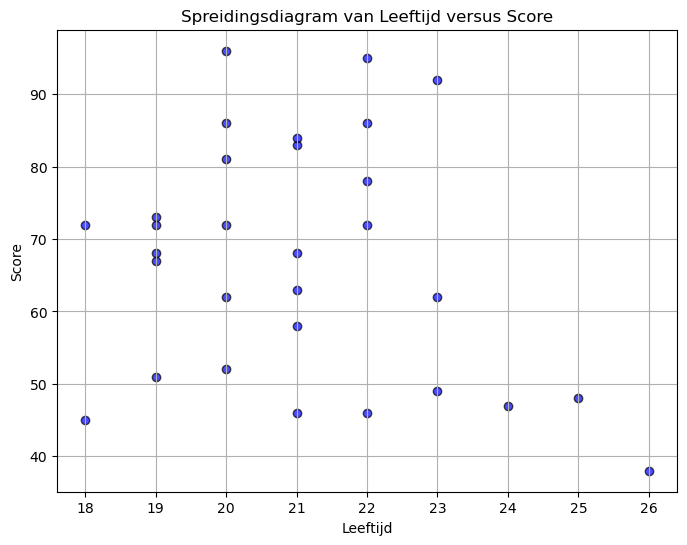
\includegraphics{opg1.7f.png}
            }
        \end{center}
    }
\end{enumerate}